%
% teil2.tex -- Beispiel-File für teil2 
%
% (c) 2020 Prof Dr Andreas Müller, Hochschule Rapperswil
%
\section{Frequenzmodulation und Bessel-Funktionen
\label{fm:section:proof}}
\rhead{Frequenzmodulation und Bessel-Funktionen}
Die momentane Trägerkreisfrequenz \(\omega_i\), wie schon in (ref) beschrieben ist, bringt die Ableitung \(\frac{d \varphi(t)}{dt}\) mit sich.
Diese wiederum kann durch \(\beta\sin(\omega_mt)\) ausgedrückt werden, wobei es das modulierende Signal \(m(t)\) ist.
Somit haben wir unser Signal
\[
x_c(t)
=
\cos(\omega_c t+\beta\sin(\omega_mt)),
\]
welches nun als Superposition von harmonischen Schwingungen
geschrieben werden soll, damit man das Frequenzspektrum ablesen 
kann.

\begin{satz}
\label{fm:satz:spektrum}
Das frequenzmodulierte Signal $x_c(t)$ lässt sich schreiben als
\begin{align}
    x_c(t)
    = 
    \cos(\omega_ct+\beta\sin(\omega_mt))
    &=
    \sum_{k= -\infty}^\infty J_{k}(\beta) \cos((\omega_c+k\omega_m)t).
    \label{fm:eq:proof}
\end{align}
\end{satz}

\subsection{Herleitung}
Zum Beweise von Satz~\ref{fm:satz:spektrum} werden zunächst einige
Hilfsmittel gebraucht, deren Anwendung später die Darstellung
\eqref{fm:eq:proof} liefert.

\subsubsection{Hilfsmittel}
Wir brauchen die Hilfe der Additionstheoreme 
\begin{align}
    \cos(A + B) 
    &= 
    \cos(A)\cos(B)-\sin(A)\sin(B)
    \label{fm:eq:addth1}
    \\
    2\cos (A)\cos (B)
    &=
    \cos(A-B)+\cos(A+B)
    \label{fm:eq:addth2}
    \\
    2\sin(A)\sin(B)
    &=
    \cos(A-B)-\cos(A+B)
    \label{fm:eq:addth3}
\end{align}
und die drei Bessel-Funktionsidentitäten,
\begin{align}
    \cos(\beta\sin\phi)
    &=
    J_0(\beta) + 2\sum_{k=1}^\infty J_{2k}(\beta) \cos(2k\phi)
    \label{fm:eq:besselid1}
    \\
    \sin(\beta\sin\phi)
    &=
    2\sum_{k=0}^\infty J_{2k+1}(\beta) \cos((2k+1)\phi)
    \label{fm:eq:besselid2}
    \\
    J_{-n}(\beta) &= (-1)^n J_n(\beta)
    \label{fm:eq:besselid3}
\end{align}
welche man im Kapitel~\ref{buch:chapter:fourier}
als Gleichungen
\eqref{buch:fourier:eqn:expinphireal},
\eqref{buch:fourier:eqn:expinphiimaginary},
und \eqref{buch:fourier:eqn:symetrie} findet.

\subsubsection{Anwenden des Additionstheorem}
Mit dem \eqref{fm:eq:addth1} wird aus dem modulierten Signal
\[
    x_c(t) 
    =
    \cos(\omega_c t + \beta\sin(\omega_mt))
    =
    \underbrace{
	\cos(\omega_c t)\cos(\beta\sin(\omega_m t))
    }_{\displaystyle=c(t)}
     -
    \underbrace{
	\sin(\omega_ct)\sin(\beta\sin(\omega_m t))
    }_{\displaystyle=s(t)}.
    \label{fm:eq:start}
\]
Die beiden Terme auf der rechten Seite werden jetzt unabhängig 
voneinander analysiert.

\subsubsection{Cosinus-Teil}
Zu Beginn wird der Cosinus-Teil
\begin{align}
    c(t) 
    &=
    \cos(\omega_c t)\cdot\cos(\beta\sin(\omega_mt))  
\notag
\intertext{mit Hilfe der Bessel-Indentität \eqref{fm:eq:besselid1} zum}
    &=
    \cos(\omega_c t) \cdot \bigg[ J_0(\beta)
    +
    2\sum_{k=1}^\infty J_{2k}(\beta) \cos( 2k \omega_m t)\, \bigg]
\notag
    \\
    &=
    J_0(\beta) \cdot \cos(\omega_c t)
    +
    \sum_{k=1}^\infty J_{2k}(\beta)
	\underbrace{
		2\cos(\omega_c t)\cos(2k\omega_m t)
	}_{\displaystyle\text{Additionstheorem \eqref{fm:eq:addth2}}},
\notag
\intertext{wobei mit dem Additionstheorem \eqref{fm:eq:addth2}
\(A = \omega_c t\) und \(B = 2k\omega_m t \) ersetzt wurden.
Nun kann die Summe in zwei Summen }
    &=
    J_0(\beta) \cdot \cos(\omega_c t)
    +
    \sum_{k=1}^\infty J_{2k}(\beta) \cos((\omega_c - 2k \omega_m) t)
    +
    \cos((\omega_c + 2k \omega_m) t) \}
    \\
    &=
    \sum_{k=1}^{\infty} J_{2k}(\beta) \cos((\omega_c - 2k \omega_m) t) 
    +
    J_0(\beta)\cdot \cos(\omega_c t) 
    +
    \sum_{k=1}^\infty J_{2k}(\beta)\cos((\omega_c + 2k \omega_m) t) 
\notag
\intertext{aufgeteilt werden.
Damit man die beiden Summen in eine zusammenfassen kann, müssen
die Kosinus-Terme in die gleiche Form gebracht werden.
Dazu kann man $k$ durch $-k$ ersetzen, dann muss in der ersten Summe
aber von $-1$ bis $-\infty$ summiert werden.
Ausserdem ist nach Bessel-Indentität \eqref{fm:eq:besselid3}
für gerade Ordnung der Besselfunktion $J_{-2k}(\beta)=J_{2k}(\beta)$,
so dass die Summe
}
    &=
    \sum_{k=-\infty}^{-1}
	J_{2k}(\beta)
	\cos\bigl((\omega_c + 2k \omega_m) t\bigr) 
    +
    J_0(\beta)\cdot \cos\bigl((\omega_c + 0\omega_m) t\bigr)
    +
    \sum_{k=1}^\infty
	J_{2k}(\beta)
	\cos\bigl((\omega_c + 2k \omega_m) t\bigr) 
\notag
\\
    &=
    \sum_{k=-\infty}^\infty
	J_{2k}(\beta)
	\bigl(\cos(\omega_c + 2k\omega_m)t\bigr).
\notag
\intertext{Dies kann vereinfacht als}
    &=
    \sum_{\text{$n$ gerade}}
	J_{n}(\beta)
	\cos\bigl((\omega_c + n \omega_m) t\bigr)
    \label{fm:eq:gerade}
\end{align}
geschrieben werden.

\subsubsection{Sinus-Teil}
Nun zum zweiten Teil der Summe \eqref{fm:eq:start}, den Sinus-Teil
\begin{align}
    s(t) 
    &=
    -\sin(\omega_c t)\cdot\sin\bigl(\beta\sin(\omega_m t)\bigr).
\notag
\intertext{Dieser wird mit der \eqref{fm:eq:besselid2} Bessel-Indentität zu}
    &=
    -\sin(\omega_c t) \cdot \bigg[
	2 \sum_{k=0}^\infty
	J_{ 2k + 1}(\beta)
	\cos\bigl(( 2k + 1) \omega_m t\bigr)
    \bigg]
    \\
    &=
    \sum_{k=0}^\infty
	-1 \cdot J_{2k+1}(\beta)
	2\sin(\omega_c t)
	\cos\bigl((2k+1)\omega_m t\bigr).
\notag
\intertext{\(2k + 1\) durchläuft alle ungeraden positiven Ganzzahlen.
Nach der Bessel-Identität \eqref{fm:eq:besselid3} ist
\(J_{-(2k+1)}(\beta) = -1\cdot J_{2k+1}(\beta)\).
Damit kann die Summe schreiben als eine Summe über die ungeraden Zahlen $n$:
}
    &=
    \sum_{\text{$n>0$ ungerade}}^\infty
	J_{-n}(\beta)
	\underbrace{
		2\sin(\omega_c t)\cos(n \omega_m t)
	}_{\displaystyle\text{Additionstheorem \eqref{fm:eq:addth3}}}.
\notag
\intertext{Auch hier wird ein Additionstheorem \eqref{fm:eq:addth3}
gebraucht, dabei ist \(A = \omega_c t\) und \(B = n \omega_m t \), 
und es entsteht:}
    &=
    \sum_{\text{$n>0$ ungerade}}
	J_{-n}(\beta)
	\{
	\cos\bigl((\omega_c - n\omega_m) t\bigr)
	-
	\cos\bigl((\omega_c + n\omega_m) t\bigr)
	\}.
\notag
\intertext{Wieder ersetzen wir $n$ durch $-n$ in der ersten Summe,
um die gleichen Kosinus-Terme zu erhalten:}
    &=
    \sum_{\text{$n<0$ ungerade}}
	J_{n}(\beta)
	\cos\bigl((\omega_c + n \omega_m) t\bigr)
    -
    \sum_{\text{$n>0$ ungerade}}
	J_{-n}(\beta)
	\cos\bigl((\omega_c + n\omega_m) t\bigr)
\notag
\\
    &=
    \sum_{\text{$n<0$ ungerade}}
	J_{n}(\beta)
	\cos\bigl((\omega_c + n \omega_m) t\bigr)
    +
    \sum_{\text{$n>0$ ungerade}}
	J_{n}(\beta)
	\cos\bigl((\omega_c + n\omega_m) t\bigr)
\notag
\intertext{
In der zweiten Gleichung haben wir wieder die
Bessel-Identität $J_{-n}(\beta)=-J_{n}(\beta)$
verwendet, die für $n$ ungerade gilt.
Jetzt kann man die beiden Summen wieder zusammenfassen in
eine einzige, die über alle positiven und negativen ungeraden
Zahl läuft:}
    &=
    \sum_{\text{$n$ ungerade}}
	J_{n}(\beta)
	\cos\bigl((\omega_c + n \omega_m) t\bigr).
\label{fm:eq:ungerade}
\end{align}

\subsubsection{Summe zusammenführen}
Beide Teile \eqref{fm:eq:gerade} für die geraden Terme 
\begin{align*}
c(t)
&=
    \sum_{n\, \text{gerade}}
	J_{n}(\beta)
	\cos\bigl((\omega_c + n\omega_m) t\bigr)
\intertext{und \eqref{fm:eq:ungerade} für die ungeraden Terme }
s(t)
&=
    \sum_{n\, \text{ungerade}}
	J_{n}(\beta)
	\cos\bigl((\omega_c + n\omega_m) t\bigr)
\intertext{ergeben zusammen}
x_c(t)
&=c(t)+s(t)
\\
&=
    \cos\bigl(\omega_ct+\beta\sin(\omega_mt)\bigr)
    =
    \sum_{k= -\infty}^\infty
	J_{n}(\beta)
	\cos\bigl((\omega_c+ n\omega_m)t\bigr).
\end{align*}
Somit ist \eqref{fm:eq:proof} bewiesen.

\subsection{Bessel-Funktionen und Frequenzspektrum}
Die Fouriertransformierte des FM-Signals
setzt sich nach Satz~\ref{fm:satz:spektrum} aus einzelnen
Termen zusammen, die mit Werten von Bessel-Funktionen
gewichtet sind.
Um die Verbindung zur Berechnung des Spektrums im Falle
der Amplitudenmodulation herzustellen, schreiben wir
das modulierte Signal
%Nochmals zur erinnerung sah unser Träger Signal anfangs so aus:
%\(x_c(t) = A_c \cdot \cos(\omega_c(t)+\varphi)\), dabei modulierten
%wir den parameter \( \varphi = \beta\sin(\omega_mt) \).
%Davon sahen wir das sich ursprünglich unser Signal
%\(m_{FM}(t) = \cos(\omega_m t)\) war. 
%Wie das Beat zusammenhängt sieht man im Abschnitt ( ref). 
\[
x_{\text{FM}}(t)
= 
\sum_{k= -\infty}^\infty J_{n}(\beta) \cos((\omega_c+ n\omega_m)t).
\]
wieder in komplexer Form als
%Diese Summe nun Fourier Transformiert ergibt
\[
x_{\text{FM}}(t)
= 
\sum_{k= -\infty}^\infty
J_{n}(\beta) \cdot \frac{1}{2}
\left(e^{j(\omega_c+ n\omega_m)t}\;+\; e^{-j(\omega_c+ n\omega_m)t}\right).
\]
Im Frequenzbereich entsteht also wieder bezüglich $0$ symmetrisch
angeordnete Dirac-Impulse bei den Kreisfrequenzen $\pm(\omega_c+n\omega_m)$
mit dem Gewicht $J_n(\beta)$.
Die Abbildung~\ref{fig:bessel} zeigt die Funktionswerte der
Besselfunktionen $J_n$ in Abhängigkeit von $\beta$.
%Gegenüber AM hat sich bei FM das Spektrum zu einer Summe mit
%Gewichtungen durch Werte der Bessel-Funktionen verändert.
\begin{figure}
\centering
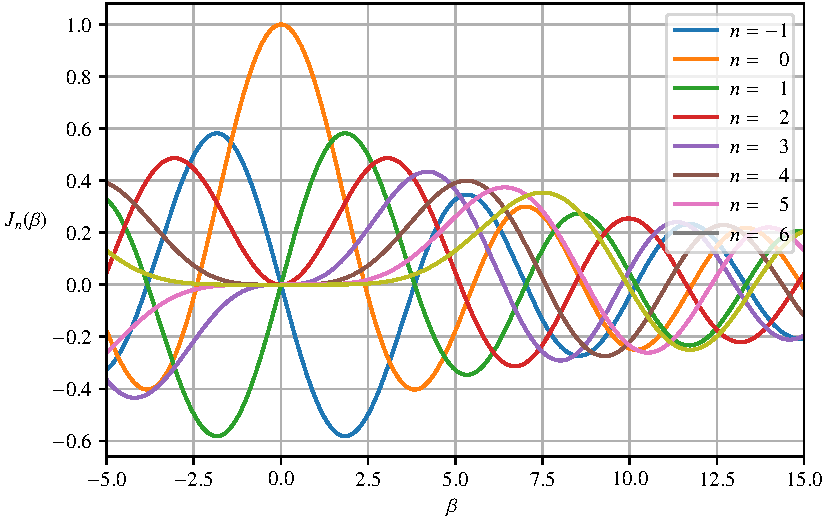
\includegraphics{papers/fm/images/bessel.pdf}
\caption{Bessel-Funktion \(J_{n}(\beta)\)}
\label{fig:bessel}
\end{figure}

\subsubsection{Kleine Werte von $\beta$}
Die Bessel-Funktionen $J_n$ haben für $n>0$ eine Nullstelle.
Für kleine Werte von $\beta$ sind daher auch die Werte $J_n(\beta)$ 
klein.
Der dominierende Term im Frequenzspektrum ist $J_0(\beta)$, der nur den Träger
wiedergibt.
Da die Nullstelle bei $0$ mit zunehmendem $n$ immer höhere Ordnung hat,
werden die Werte $J_n(\beta)$ mit $\beta^n$ gegen  0 gehen, es
sind also nur wenige Terme nötig, um das Spektrum mit ausreichender
Genauigkeit wiederzugeben.

%Hier sieht man gut das für kleine \( \beta \lessgtr \) nur die
%ersten Summanden \( n\) zuständig sind.
%%
%So kann man mit dem \(\beta\) gut bestimmen bis wo die Summe berchnet
%werden soll. 

\subsubsection{Symmetrie}
Für Bessel-Funktionen mit negativer Ordnung \(-n\) gilt die
Beziehung
\[
    J_{-n} (\beta) = (-1)^n \cdot J_n (\beta) = J_n (-\beta).
    \label{fm:eq:besselid:gerad:ungerade}
\]
Zur Illustration wurde in Abbildung \ref{fig:bessel} auch ein Abschnitt
von \(J_n (-\beta)\) dargestellt.
Man erkennt daraus, dass für gerade Ordnungen \(n\) die Bessel-Funktion
erster Art eine gerade Funktion ist 
(d.h. \(J_n (-\beta) = J_n (\beta))\) und damit
\(J_{-n} (\beta) = J_n (\beta)\) gilt.
Für ungerade Ordnungen n ist die Bessel-Funktion erster Art eine
ugnerade Funktion 
(d.h. \(J_n (-\beta) = -J_n (\beta)\)), womit gleichzeitig
\(J_{-n} (\beta) = -J_n (\beta)\) gilt.

\subsubsection{Beispiel}
Für ein Beispiel nehmen wir
\(\beta = 1 [\text{rad}]\), \(\omega_m = 2 \pi \cdot 20 [\text{Hz}]\),
\(\omega_c =  2 \pi \cdot 100 [\text{Hz}] \).
Dann sieht \(x_{FM}(t)\) im Frequenzbereich wie in
Abbildung~\ref{fig:fm:bessel_fm} aus, durch die Bessel-Koeffizenten bei
\(\beta = 1\) kann man die Peaks im Frequenzbereich bestimmen.
Hier wurden sie noch mit einem Faktor \(\pi\) skaliert.
\begin{figure}
\centering
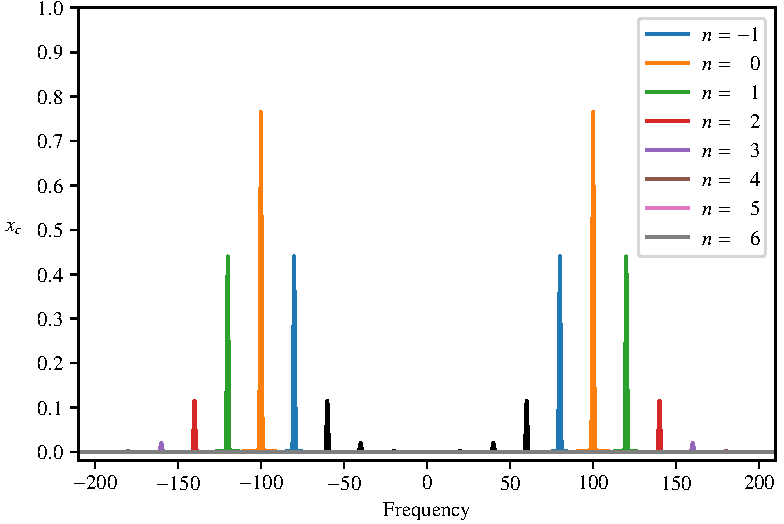
\includegraphics{papers/fm/images/normal.pdf}
\caption{Beispiel eines FM Übertragenen Signal}
\label{fig:fm:bessel_fm}
\end{figure}
Nun verändern wir die drei Parameter \(\beta \,\omega_c \,\omega_m \)
und sehen was sich verändern wird.

\subsubsection{Veränderung von $\bm{\beta}$}
Da \(\beta\) in keiner Abhängigkeit von den anderen Parametern steht,
und jegliglich die Anzahl der nötigen Summanden bestimmt.
So wird es auch diese Anzahl bestimmen dies bei der
Abbildung~\ref{fig:fm:beta_fm} ersichtlich ist.
\begin{figure}[h]
	\centering
	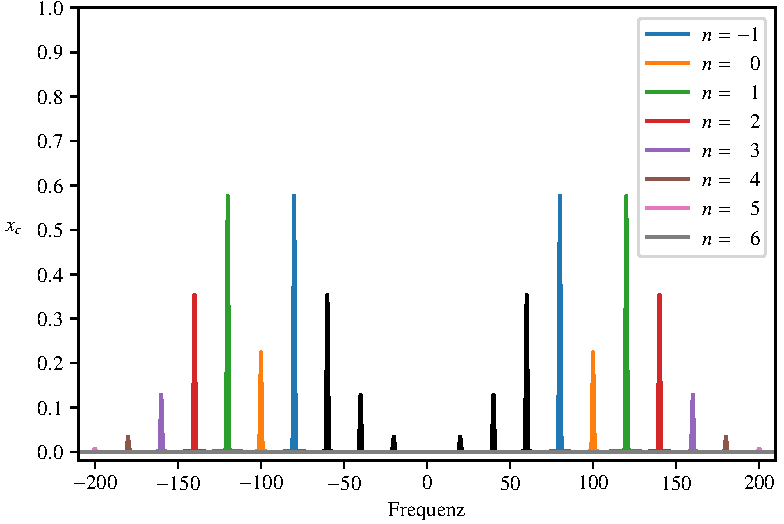
\includegraphics{papers/fm/images/beta2.pdf}
	\caption{Veränderung durch \(\beta\)}
	\label{fig:fm:beta_fm}
\end{figure}

\subsubsection{Veränderung von $\bm{\omega_c}$}
Dies ist die Trägerfrequenz, auf die unser Signal aufmoduliert wurde.
Sie bestimmt die Frequenz bei welcher das Signal gefunden werden kann. 
Ändern wir es von \( 100\,[\text{Hz}] \) auf \(150\,[\text{Hz}]\),
dann zeigt
Abbildung~\ref{fig:fm:fc_150}, wie sich das Spektrum verschiebt.
\begin{figure}[h]
	\centering
	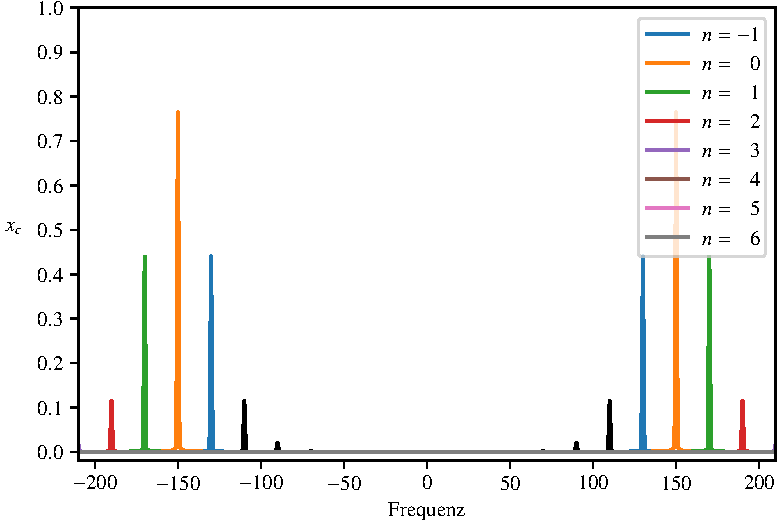
\includegraphics{papers/fm/images/fc150.pdf}
	\caption{Veränderung durch \(\omega_c\)}
	\label{fig:fm:fc_150}
\end{figure}

\subsubsection{Veränderung von $\bm{\omega_m}$}
Bei Amplitudenmodulation bestimmt dieser Parameter
die Bandbreite um das Trägersignal, innerhalb
der das modulierte Signal \(x_{AM}\) gefunden werden kann.
Auch bei Frequenzmodulation ist er ein Mass für die Bandbreite,
allerdings bestimmt die Grösse von $\beta$, wieviele Vielfache
der Frequenz $\omega_m$ berücksichtigt werden müssen, um das
Signal ausreichend genau wiederzugeben.
Ein kleineres $\omega_m$ bewirkt, dass Frequenzen im Spektrum näher
bei der Trägerfrequenz liegen, aber ansonsten die gleichen
Gewichte $J_n(\beta)$ haben, die nur von $\beta$ abhängen.
Dies ist in Abbildung~\ref{fig:fm:fm_10} dargestellt.. 
In dieser Abbildung wurde die Modulation von \(20 [\text{Hz}]\) auf
\( 10[\text{Hz}]\) verkleinert, und somit auch gestaucht. 
\begin{figure}[h]
	\centering
	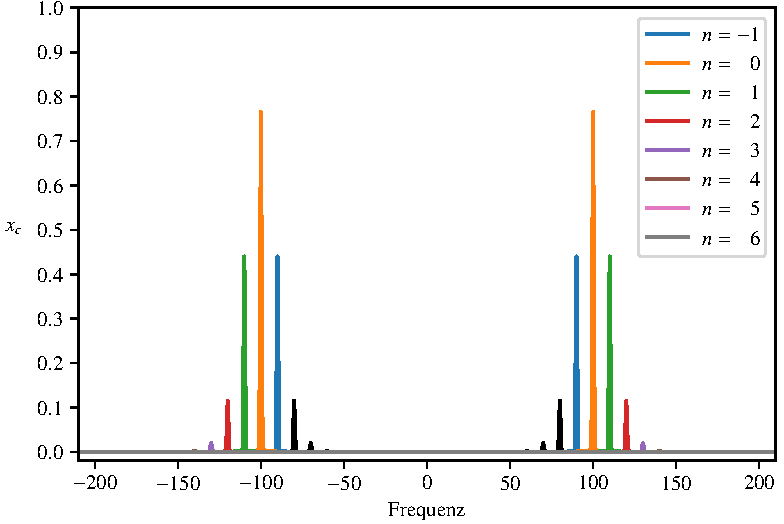
\includegraphics{papers/fm/images/fm10.pdf}
	\caption{Veränderung durch \(\omega_m\)}
	\label{fig:fm:fm_10}
\end{figure}






